\chapter{Lecture 8}
\section{Model to Model}
In the last lecture, we covered the process of mapping models to models. IN particular, we covered asymptotic analysis. We looked at equations of the form
\begin{align} \label{eqn:asympt}
    f(u_{\epsilon}, \epsilon) = 0
\end{align}
and investigated the form of $u_{\epsilon}$ as $\epsilon \to 0$. This perturbation falls into two categories, regular perturbations and singular perturbations. Regular perturbations are such that
\begin{align} \label{eqn:regperturb}
f(u_{0}, 0) = 0
\end{align}
is a well-defined problem for whatever boundary condition we have for Equation \ref{eqn:asympt}. Singular perturbations have ill-posedness, and a choice of boundary condition for the limiting equation must be made. Consider
\begin{align} \label{eqn:singularex}
\pm \epsilon u_{xx} - u_{x} = 0.
\end{align}
We saw in the previous lecture that the sign chosen on the first term in Equation \ref{eqn:singularex} influences the form of the limiting form expressed in Equation \ref{eqn:regperturb}. Let us now consider yet another example below.
\begin{ceqn} \label{eqn:singex2}
\epsilon u_{xx} + u &= 0 \\
u(0)&=0, u(1) = 1
\end{ceqn}
We get a solution of the form
\begin{align} \label{eqn:singex2soln}
u_{\epsilon}(x) = sin\left(\sqrt{\frac{1}{\epsilon}} x\right).
\end{align}
Furthermore, this solution only solves the boundary right-endpoint boundary condition when $\sqrt{\epsilon} = \frac{2n}{\pi}$ for $n \in \mathbb{N}$. So taking $\epsilon \to 0$ must be restricted much more stringently to taking $n \to \infty$ and considering only $\epsilon_{n} = \left(\frac{2n}{\pi}\right)^{2}$. However, even if we take this limit only in this sense, then we have
\begin{align} \label{eqn:singex2soln2}
    \phi_{n}(x) :&= u_{\left(\frac{2n}{\pi}\right)^2}(x) \\
    &= sin\left(\frac{2nx}{\pi}\right).
\end{align}
But $\phi_n$ does not converge as $n \to \infty$ except for at $x=0$. So a limiting solution cannot be recovered in any sense for this case! 

\askbjorn{Remark expansion}

\subsection{Generalization of Asymptotic Analysis to PDE}
We consider an advection-diffusion equation give below.
\begin{ceqn} \label{eqn:singadvect}
u_{t} + u_{x} &= \epsilon u_{xx} \\
u(x,0) = u_{0}(x) & t > 0, 0<x<1 \\
u(0,t) = u_{L}(t) & u(1,t) = u_{R}(t)
\end{ceqn}

\begin{figure}
    \centering
    
\includegraphics{images/x.pdf}
    \caption{Refer to figure in notes}
    \label{fig:my_label}
\end{figure}

\subsubsection{Prandtl Boundary Layer Equations}
We consider now the Prandtl Boundary Layer Equations for incompressible fluid flow. \askbjorn{This is extensive, we nee dto come back to it later.}

\subsubsection{Averaging of Dynamical Systems (ODE)}
Consider the ODE below.
\begin{ceqn} \label{eqn:avgdyn}
u_{t} &= 1 + sin\left(\frac{t}{\epsilon}\right) \\
u(0) &= 0.
\end{ceqn}
What is the behavior of the solution as $\epsilon \to 0$ and does this limiting function solve a limiting ODE? We can explicitly construct the solution to be
\begin{align} \label{eqn:avgdynsoln}
u_{\epsilon}(t) = t - \epsilon cos\left( \frac{t}{\epsilon} \right) + \epsilon.
\end{align}
Therefore, we have for any $t > 0$, 
\begin{align} \label{eqn:avgdynlimit}
\lim_{\epsilon \to 0} u_{\epsilon}(t) = t := \bar{u}(t).
\end{align}

\begin{figure}
    \centering
    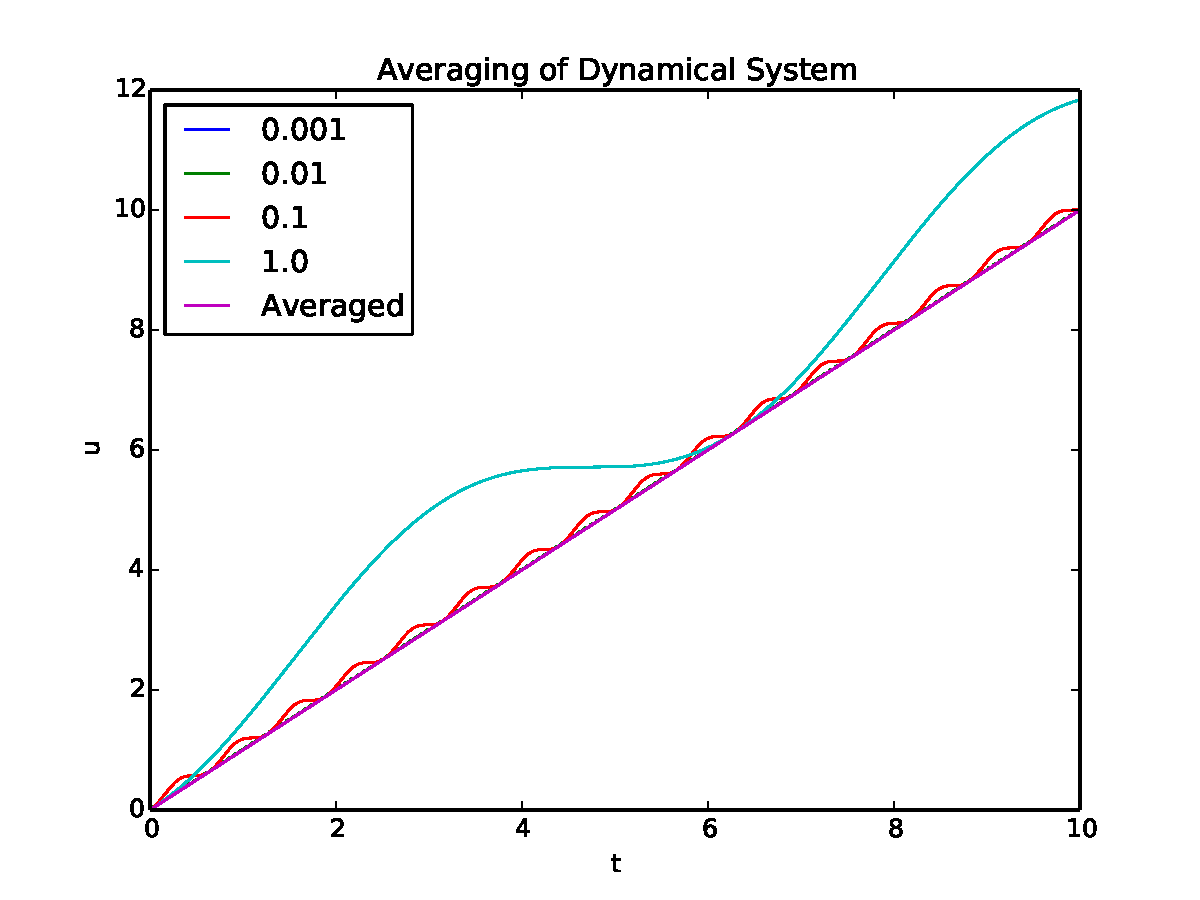
\includegraphics[width=\textwidth]{images/averaging.pdf}
    \caption{We see that as $\epsilon \to 0$, the oscillations lead to smaller and smaller discrepancy between the averaged and perturbed models}
    \label{fig:avgdynill}
\end{figure}

Qualitatively, this tells us that our solution is looks like the function $u_{\epsilon} = \bar{u} + p_{\epsilon}(t)$ where $p_{\epsilon}$ is an oscillatory term. As $\epsilon \to 0$, the oscillations matter less and less. This can be seen in Figure \ref{fig:avgdynill}. 

\subsection{Averaging of Coupled Dynamical System}
Here we consider a more complicated example. Consider the following coupled system of ODEs. 
\begin{align} \label{eqn:avgdyncoupled}
u_{t} &= v^2 & u(0) = 0 \label{eqn:top} \\
v_{t} &= \frac{1}{\epsilon} w & v(0) = 0 \label{eqn:middle} \\
w_{t} &= -\frac{1}{\epsilon} v & w(0) = 1 \label{eqn:bottom}
\end{align}
Note that we can decouple Equations \ref{eqn:middle} and \ref{eqn:bottom} and obtain harmonic oscillator models. The decoupling is achieved simply by differentiating both sides of each equation and substituting each of them into each other. Equation \ref{eqn:middle} becomes
\begin{ceqn} \label{eqn:middleuncoupled}
v_{tt} &= -\frac{1}{\epsilon^2} v \\
v(0) &= 0
\end{ceqn}
Equation \ref{eqn:bottom} becomes
\begin{ceqn} \label{eqn:bottomuncoupled}
w_{tt} &= -\frac{1}{\epsilon^2} w \\
u(0) &= 1
\end{ceqn}
We recover $v(t) = sin\left(\frac{t}{\epsilon}\right)$ and $w(t) = cos\left( \frac{t}{\epsilon} \right)$. Plugging these results and plugging into Equation \ref{eqn:top} and using trig identities, we obtain
\begin{align} \label{eqn:avgdyncoupledsoln}
u_{\epsilon}(t) = \frac{1}{2}\left(t - \frac{\epsilon}{2} sin\left(\frac{2t}{\epsilon}\right)\right).
\end{align}
We again take $\epsilon \to 0$ to get
\begin{align} \label{eqn:avgdyncoupledlimit}
\lim_{\epsilon \to 0} u_{\epsilon}(t) = \frac{t}{2} := \bar{u}(t).
\end{align}
Furthermore, we can derive a limiting differential equation as 
\begin{align} \label{eqn:avgdynlimiteqn}
u_{t} &= \frac{1}{2} \\
u(0) &= 0
\end{align}
This is a valid limiting equation that preserves all limits that we would like. However, the auxiliary variables $v$ and $w$ \textbf{do not have limiting equations!} Furthermore, if we were to average $v$ and $w$ before we were to plug them into Equation \ref{eqn:top}, then this would not work. It is thus important in this example that when we say ``limiting equation,'' we mean that we only take average as $\epsilon \to 0$ in Equation \ref{eqn:top}  with no other limits taken first. This example illustrates that we sometimes need to be careful in how we define limiting equations so that what we mean by ``asymptotic'' or ``averaging'' may need to be precisely defined to avoid misinterpretation of our limiting solution and/or limiting equation.

As a remark, we may note that $v^2 + w^2 = 1$ and is thus an invariant. As $\epsilon \to 0$, we simply observe that the solutions ``spin'' faster and faster around the unit circle.

We conclude this lecture by noting that the argument outlined here for this simple harmonic oscillator case can be generalized to the following equation.
\begin{ceqn} \label{eqn:avgdyncoupledgen}
u_{t}^{\epsilon} &= f(u^{\epsilon}, v^{\epsilon}) \\
v_{t}^{\epsilon} &= \frac{1}{\epsilon} g(u^{\epsilon}, v^{\epsilon}
\end{ceqn}
For fixed $u^{\epsilon}$, $v^{\epsilon}$ defines an invariant measure, albeit possibly more abstract than our previous case on the unit circle. From this we can recover that $u^{\epsilon} \to u$ where $u$ is the solution to
\begin{ceqn} \label{eqn:avgdyncoupledgenlimit}
u_{t} &= F(u) \\
F(u) := \int f(u,v) d\mu_{v}
\end{ceqn}
where $\mu_{v}$ is the invariant measure defined for fixed $u$. \askbjorn{Expand or leave here?}